\section{Detail Design}
\subsection{Visitor Pattern}
In object-oriented programming and software engineering, the visitor design pattern is a way of separating an algorithm from an object structure on which it operates. A practical result of this separation is the ability to add new operations to extant object structures without modifying the structures. It is one way to follow the open/closed principle.\\
In essence, the visitor allows adding new virtual functions to a family of classes, without modifying the classes. Instead, a visitor class is created that implements all of the appropriate specializations of the virtual function. The visitor takes the instance reference as input, and implements the goal through double dispatch.
\subsubsection{Definition}
The Gang of Four defines the Visitor as:\\
Represent an operation to be performed on elements of an object structure. Visitor lets you define a new operation without changing the classes of the elements on which it operates.\\
The nature of the Visitor makes it an ideal pattern to plug into public APIs thus allowing its clients to perform operations on a class using a “visiting” class without having to modify the source.
\begin{figure}[H]
	\centering
	\includegraphics{images/visitor_pattern.png}
	\caption{Visitor Pattern}
\end{figure}
\subsubsection{Motivation}
Consider the design of a 2D computer-aided design (CAD) system. At its core there are several types to represent basic geometric shapes like circles, lines, and arcs. The entities are ordered into layers, and at the top of the type hierarchy is the drawing, which is simply a list of layers, plus some added properties.\\
A fundamental operation on this type hierarchy is saving a drawing to the system's native file format. At first glance it may seem acceptable to add local save methods to all types in the hierarchy. But it is also useful to be able to save drawings to other file formats. Adding ever more methods for saving into many different file formats soon clutters the relatively pure original geometric data structure.\\
A naive way to solve this would be to maintain separate functions for each file format. Such a save function would take a drawing as input, traverse it, and encode into that specific file format. As this is done for each added different format, duplication between the functions accumulates. For example, saving a circle shape in a raster format requires very similar code no matter what specific raster form is used, and is different from other primitive shapes. The case for other primitive shapes like lines and polygons is similar. Thus, the code becomes a large outer loop traversing through the objects, with a large decision tree inside the loop querying the type of the object. Another problem with this approach is that it is very easy to miss a shape in one or more savers, or a new primitive shape is introduced, but the save routine is implemented only for one file type and not others, leading to code extension and maintenance problems.\\
Instead, the Visitor pattern can be applied. It encodes a logical operation on the whole hierarchy into one class containing one method per type. In the CAD example, each save function would be implemented as a separate Visitor subclass. This would remove all duplication of type checks and traversal steps. It would also make the compiler complain if a shape is omitted.\\
Another motive is to reuse iteration code. For example, iterating over a directory structure could be implemented with a visitor pattern. This would allow creating file searches, file backups, directory removal, etc., by implementing a visitor for each function while reusing the iteration code.
\subsubsection{Details}
The visitor pattern requires a programming language that supports single dispatch. Under this condition, consider two objects, each of some class type; one is termed the element, and the other is visitor. An element has an accept method that can take the visitor as an argument. The accept method calls a visit method of the visitor; the element passes itself as an argument to the visit method. Thus:\\
\begin{itemize}
	\item When the accept method is called in the program, its implementation is chosen based on both:
	\begin{itemize}
		\item The dynamic type of the element
		\item The static type of the visitor.
	\end{itemize}
	\item When the associated visit method is called, its implementation is chosen based on both:
	\begin{itemize}
		\item The dynamic type of the visitor.
		\item The static type of the element as known from within the implementation of the accept method, which is the same as the dynamic type of the element. (As a bonus, if the visitor can't handle an argument of the given element's type, then the compiler will catch the error.)
	\end{itemize}
	\item Thus, the implementation of the visit method is chosen based on both:
	\begin{itemize}
		\item The dynamic type of the element.
		\item The dynamic type of the visitor.
	\end{itemize}
\end{itemize}
This effectively implements double dispatch. For languages which object systems support multiple dispatch, not only single dispatch, such as Common Lisp, implementing the visitor pattern in them is trivial.\\
In this way, one algorithm can be written to traverse a graph of elements, and many different kinds of operations can be performed during that traversal by supplying different kinds of visitors to interact with the elements based on the dynamic types of both the elements and the visitors.\\
Some languages (e.g., C\# via the Dynamic Language Runtime (DLR)) support multiple dispatch, which greatly simplifies implementing the Visitor pattern (a.k.a. Dynamic Visitor) by allowing use of simple function overloading to cover all the cases being visited. A dynamic visitor, provided it operates on public data only, conforms to the open/closed principle (since it does not modify extant structures) and to the single responsibility principle (since it implements the Visitor pattern in a separate component).
\subsection{Lambda Expressions}
\subsubsection{Introduction to Lambdas}
In C++11, a lambda expression—often called a lambda—is a convenient way of defining an anonymous function object right at the location where it is invoked or passed as an argument to a function. Typically lambdas are used to encapsulate a few lines of code that are passed to algorithms or asynchronous methods. A lambda expression contains the following components:
\begin{enumerate}
	\item capture clause (Also known as the lambda-introducer in the C++ specification.)
	\item parameter list Optional. (Also known as the lambda declarator)
	\item mutable specification Optional.
	\item exception-specification Optional.
	\item trailing-return-type Optional.
	\item lambda body)
\end{enumerate}
This is shown in the following picture followed by an example:
\begin{figure}[H]
	\centering
	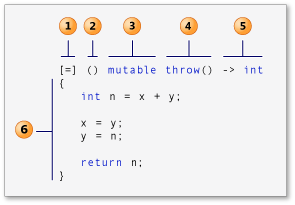
\includegraphics{images/lambda_components.png}
	\caption{Lambda expression components}
\end{figure}
\begin{figure}[H]
	\centering
	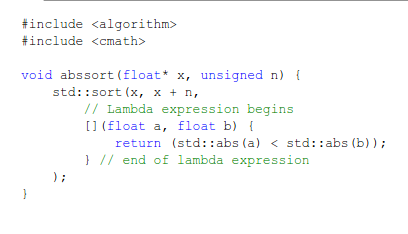
\includegraphics{images/lambda_example.png}
	\caption{Lambda expression example}
\end{figure}
\subsubsection{Benefits of using Lambdas}
Lambdas are lightweight, nameless functions that can be defined just-in-place where they are used. Lambdas didn't come to C++ as a specific-purpose feature (i.e., functional programming): the existing STL components, like the for\_each algorithm, and its new ones like <thread> or <future>, allow you to specify function arguments as lambdas beside C-like functions and functors. Unless you need a function available in more than one place, you'll feel more comfortable using lambdas as arguments of STL components.
